\section{Hanging nodes}
As the goal is automatic
mesh adaptivity on both triangular and quadrilateral (or combined) meshes, one of the important characteristics of triangulations is their regularity. This section shows why the regularity assumption should be dropped and how irregular meshes are treated.

\subsection{Hanging nodes and irregularity rules} 
\label{sec:hang}

At the beginning, let us recall the {\em red-green} refinement
strategy. This technique first subdivides desired elements
into geometrically convenient subelements with
hanging nodes and then it eliminates the
hanging nodes by forcing refinement of additional
elements. This is illustrated in Figure \ref{fig:redgreen}.
This approach preserves regularity of the mesh but in the case of triangles,
\begin{figure}[hb]
\centering
\vspace{4mm}
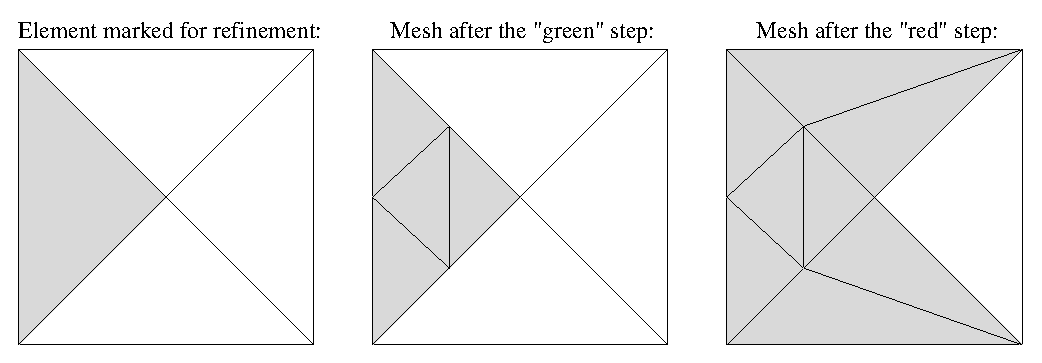
\includegraphics[width=0.9\textwidth]{img/redgreen}
\vspace{-2mm}
\caption{Red-green refinement.}
\label{fig:redgreen}
\end{figure}
it introduces elements with sharp angles
which are not desirable in finite element analysis. In the case of quadrilaterals, it also negatively influence the the element shapes.
It becomes extremely cumbersome when
repeated refinements occur  in the same part of the
domain (e.g., toward a boundary layer or point singularity).

The ``red'' refinements can be avoided
by introducing {\em hanging nodes}, i.e., by allowing
{\em irregular meshes} where element vertices lie
in the interior of edges of other elements. In order to keep the
computer implementation simple, most finite element
working with hanging nodes
limit the maximum difference of refinement
levels of adjacent elements to one (so-called
{\em $1$-irregularity rule}) --  see, e.g., \cite{demk5,RaDe2,SoDe}.
In the following, by {\em $k$-irregularity rule} (or {\em hanging nodes of level $k$})
we mean this type of restriction where the maximum
difference of refinement levels of adjacent elements
is $k$. In this context, $k=0$ corresponds to adaptivity with
regular meshes and $k=\infty$ to adaptivity with arbitrary-level
hanging nodes.

It is illustrated in Figure \ref{fig:one_irr} that even the
1-irregularity rule does not avoid all forced refinements:
\begin{figure}[h!]
\centering
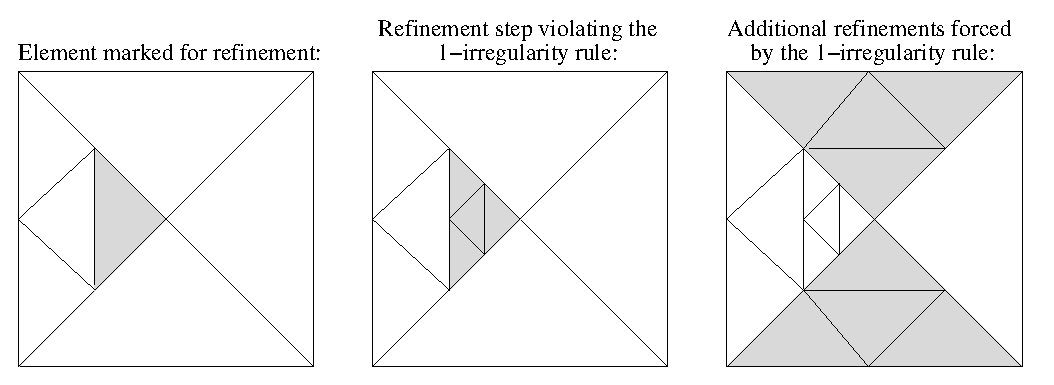
\includegraphics[width=0.9\textwidth]{img/one-irr}
\caption{Refinement with 1-irregularity rule.}
\label{fig:one_irr}
\end{figure}

The amount of forced refinements
in the mesh depends strongly on the level of hanging nodes.
Next we introduce a model problem and show that the level of
hanging nodes also influences significantly both the number of degrees of freedom and condition number of stiffness matrices.

\paragraph{Model problem}

Consider a Poisson equation $-\Delta u = f$ in $\Omega$ with $u = 0$ on
the boundary of $\Omega$, where $\Omega = (-1,1)^2$.
Assume a right-hand side $f$ such that the corresponding
exact solution $u$ is zero everywhere in $\Omega$ with the exception of
a local perturbation occuring inside of a small triangle $T_n$ with the vertices
$[-2^{-n}, -2^{-n}]$, $[0,0]$, $[-2^{-n}, 2^{-n}]$.
The domain is covered with a coarse four-element mesh shown in Figure \ref{fig:academic}.
For simplicity, all elements are equipped with a uniform polynomial degree $p \ge 1$.
\begin{figure}[h!]
\centering
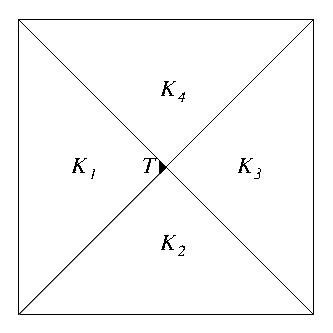
\includegraphics[width=0.26\textwidth]{img/academic}
\caption{Domain and initial mesh for the study of $k$-irregularity rules.}
\label{fig:academic}
\end{figure}

We perform the following simple experiment: Starting from the
coarse mesh shown in Figure \ref{fig:academic}, we run an adaptive algorithm
which in each step applies the ``green'' refinement to every mesh triangle
$K$ such that $K \cap T_n \not = \emptyset$ and $K \not \subset T_n$.
Figure \ref{fig:academic2} shows final meshes obtained with various
levels of hanging nodes for $n = 5$:

\begin{figure}[h!]
\centering
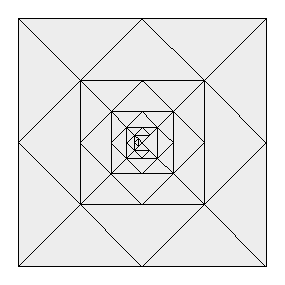
\includegraphics[width=0.24\textwidth]{img/mesh-1ir}
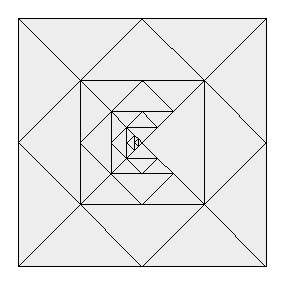
\includegraphics[width=0.24\textwidth]{img/mesh-2ir}
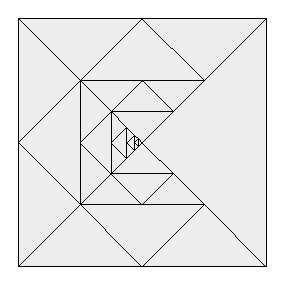
\includegraphics[width=0.24\textwidth]{img/mesh-3ir}
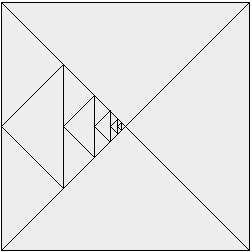
\includegraphics[width=0.24\textwidth]{img/mesh-free}
\caption{Meshes obtained with $k$-irregularity rules, $k = 1,2,3,\infty$.}
\label{fig:academic2}
\end{figure}

Notice that, since $T_n \subset K_1$, all refinements within the elements
$K_2, K_3, K_4$ are forced and they do not improve the resolution. The reader 
can see that the amount of forced refinements decreases as $k$ grows, 
vanishing completely with $k = \infty$.

Next let us choose, e.g., $p=3$, and run the same adaptive procedure for
$n = 1, 2, \ldots, 15$. Figure \ref{fig:academic3a} shows the number of degrees
of freedom corresponding to the final meshes. The horizontal axis represents
the spatial scale $2^{-n}$. 
For the same computations, Figure \ref{fig:academic3b}
shows the condition number of the corresponding stiffness matrices.

\begin{figure}[h!]
\centering
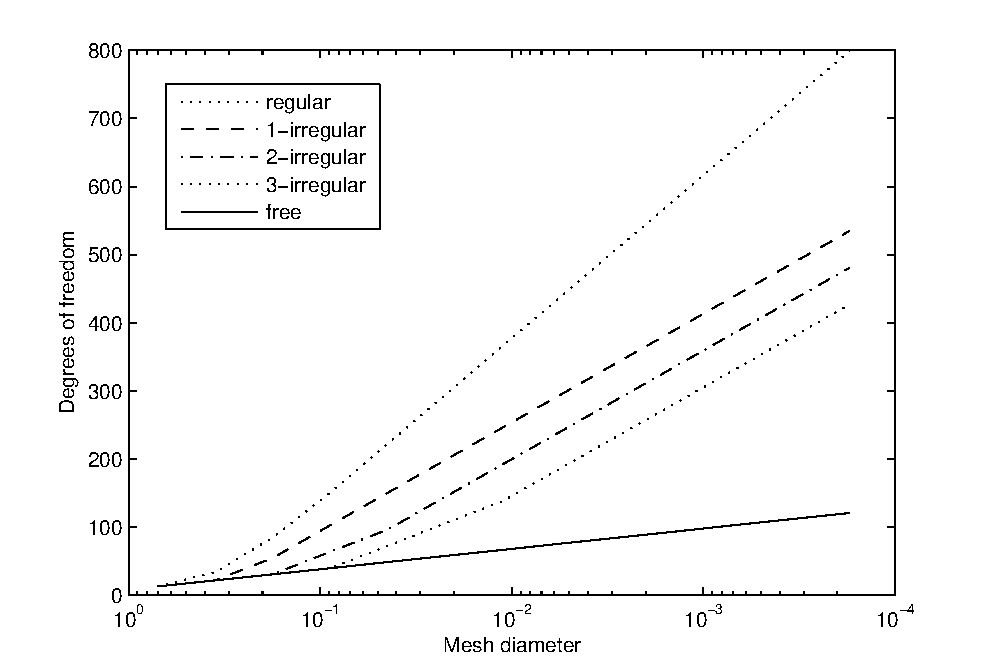
\includegraphics[width=0.9\textwidth]{img/dof-cubic}
\vspace{-4mm}
\caption{Size of the stiffness matrix for final meshes. Level of hanging
         nodes: $k = 0,1,2,3,\infty$.}
\label{fig:academic3a}
\end{figure}
\begin{figure}[h!]
\centering
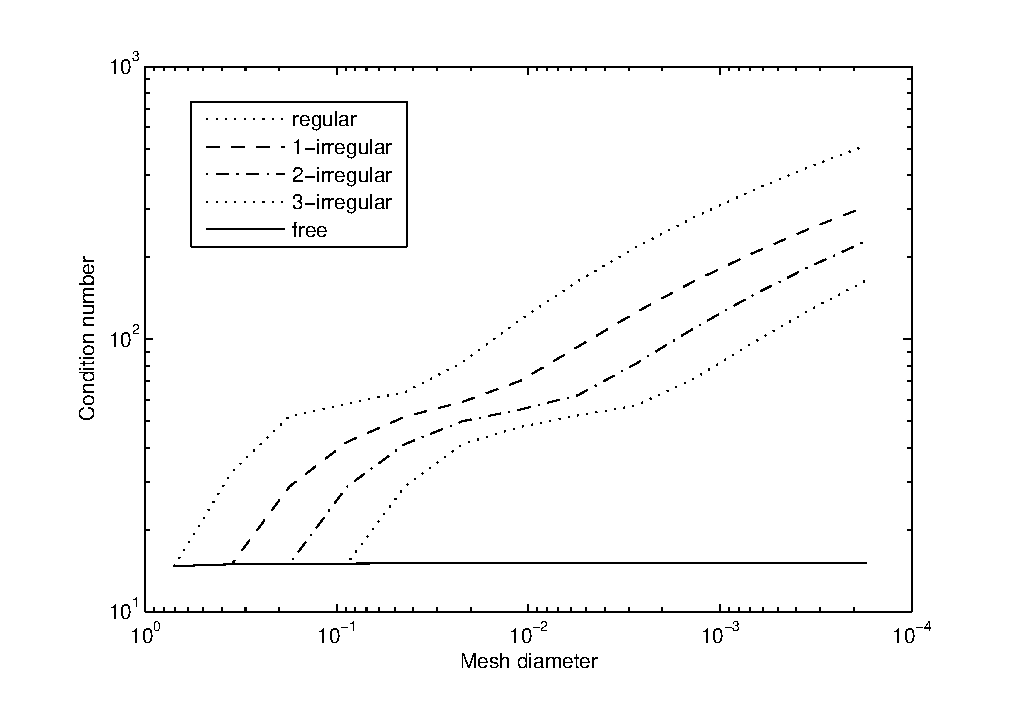
\includegraphics[width=0.9\textwidth]{img/cond-cubic}
\vspace{-4mm}
\caption{Condition number of the stiffness matrix for final meshes.
         Level of hanging nodes: $k = 0,1,2,3,\infty$.}
\label{fig:academic3b}
\end{figure}

In DGFEM, the requirement from the conforming FEM of continuity across mesh edges is dropped, and this means that we only have to be able to calculate fluxes $\bs{f}$ across mesh edges properly (as opposed to conforming finite elements, where we have to take care of the continuity requirement in vertices and on edges). With arbitrary-level hanging nodes, the flux calculation also poses a challenge, and the algorithmic treatment will be described in the section~\ref{sec:data_structures}.
